\documentclass[11pt]{report}

% Paquetes y configuraciones adicionales
\usepackage{graphicx}
\usepackage[export]{adjustbox}
\usepackage{caption}
\usepackage{float}
\usepackage{titlesec}
\usepackage{geometry}
\usepackage[hidelinks]{hyperref}
\usepackage{titling}
\usepackage{titlesec}
\usepackage{parskip}
\usepackage{wasysym}
\usepackage{tikzsymbols}
\usepackage{fancyvrb}
\usepackage{xurl}
\usepackage{hyperref}
\usepackage[spanish]{babel}
\usepackage{listings}
\usepackage{xcolor}

\newcommand{\subtitle}[1]{
  \posttitle{
    \par\end{center}
    \begin{center}\large#1\end{center}
    \vskip0.5em}
}

% Configura los márgenes
\geometry{
  left=2cm,   % Ajusta este valor al margen izquierdo deseado
  right=2cm,  % Ajusta este valor al margen derecho deseado
  top=3cm,
  bottom=3cm,
}

% Configuración de los títulos de las secciones
\titlespacing{\section}{0pt}{\parskip}{\parskip}
\titlespacing{\subsection}{0pt}{\parskip}{\parskip}
\titlespacing{\subsubsection}{0pt}{\parskip}{\parskip}

% Redefinir el formato de los capítulos y añadir un punto después del número
\makeatletter
\renewcommand{\@makechapterhead}[1]{%
  \vspace*{0\p@} % Ajusta este valor para el espaciado deseado antes del título del capítulo
  {\parindent \z@ \raggedright \normalfont
    \ifnum \c@secnumdepth >\m@ne
        \huge\bfseries \thechapter.\ % Añade un punto después del número
    \fi
    \interlinepenalty\@M
    #1\par\nobreak
    \vspace{10pt} % Ajusta este valor para el espacio deseado después del título del capítulo
  }}
\makeatother

% Configura para que cada \chapter no comience en una pagina nueva
\makeatletter
\renewcommand\chapter{\@startsection{chapter}{0}{\z@}%
    {-3.5ex \@plus -1ex \@minus -.2ex}%
    {2.3ex \@plus.2ex}%
    {\normalfont\Large\bfseries}}
\makeatother

% Configurar los colores para el código
\definecolor{codegreen}{rgb}{0,0.6,0}
\definecolor{codegray}{rgb}{0.5,0.5,0.5}
\definecolor{codepurple}{rgb}{0.58,0,0.82}
\definecolor{backcolour}{rgb}{0.95,0.95,0.92}

% Configurar el estilo para el código
\lstdefinestyle{mystyle}{
  backgroundcolor=\color{backcolour},   
  commentstyle=\color{codegreen},
  keywordstyle=\color{magenta},
  numberstyle=\tiny\color{codegray},
  stringstyle=\color{codepurple},
  basicstyle=\ttfamily\footnotesize,
  breakatwhitespace=false,         
  breaklines=true,                 
  captionpos=b,                    
  keepspaces=true,                 
  numbers=left,                    
  numbersep=5pt,                  
  showspaces=false,                
  showstringspaces=false,
  showtabs=false,                  
  tabsize=2
}

%==============================================================================
% Cosas para la documentación LateX
% % Sangría
% \setlength{\parindent}{1em}Texto

% % Quitar sangría
% \noindent

% % Punto
% \CIRCLE \ \ \textbf{Texto} \emph{algo}
% \begin{itemize}
%   \item \textbf{Negrita:} Texto
%   \item \textbf{Negrita:} Texto
% \end{itemize}

% % Introducir código
% \begin{center}
%   \begin{BVerbatim}
%     ... Código
%   \end{BVerbatim}
% \end{center}

% Poner una imagen
% \begin{figure}[H]
%   \centering
%   \includegraphics[scale=0.55]{img/}
%   \caption{Exportación de la base de datos en formato sql}
%   \label{fig:exportación de la base de datos en formato sql}
% \end{figure}

% Poner dos imágenes
% \begin{figure}[H]
%   \begin{subfigure}{0.5\textwidth}
%     \centering
%     \includegraphics[scale=0.45]{img/}
%     \caption{Texto imagen 1}
%   \end{subfigure}%
%   \begin{subfigure}{0.5\textwidth}
%     \centering
%     \includegraphics[scale=0.45]{img/}
%     \caption{Texto imagen 2}
%   \end{subfigure}
%   \caption{Texto general}
% \end{figure}

% % Poner una tabla
% \begin{table}[H]
%   \centering
%   \begin{tabular}{|c|c|c|c|}
%     \hline
%     \textbf{Campo 1} & \textbf{Campo 2} & \textbf{Campo 3} & \textbf{Campo 4} \\ \hline
%     Texto & Texto & Texto & Texto \\ \hline
%     Texto & Texto & Texto & Texto \\ \hline
%     Texto & Texto & Texto & Texto \\ \hline
%     Texto & Texto & Texto & Texto \\ \hline
%   \end{tabular}
%   \caption{Nombre de la tabla}
%   \label{tab:nombre de la tabla}
% \end{table}

%==============================================================================

\begin{document}

% Portada del informe
\title{Practica 09. Shorewall: Doble firewall con DMZ}
\subtitle{Seguridad de Sistemas Informáticos}
\author{Carlos Pérez Fino y Cheuk Kelly Ng Pante}
\date{\today}

\maketitle

\pagestyle{empty} % Desactiva la numeración de página para el índice

% Índice
\tableofcontents

% Nueva página
\cleardoublepage

\pagestyle{plain} % Vuelve a activar la numeración de página
\setcounter{page}{1} % Reinicia el contador de página a 1

% Capitulo 1
\chapter{Configuración de red con dos firewalls y tres zonas}
Esta práctica se va a realizar una configuracion de un firewall con DMZ utilizando
\emph{Shorewall} y \emph{firewalld}. Se va a implementar un diseño con doble firewall
(Interno con \emph{firewalld} y externo con \emph{Shorewall}) con dos interfaces para
gestionar las zonas de Internet, DMZ y LAN. La DMZ se localiza entre los dos firewalls 
configurados.

Se va a partir del siguiente diseño de red con dos firewalls y tres zonas:
\begin{figure}[H]
  \centering
  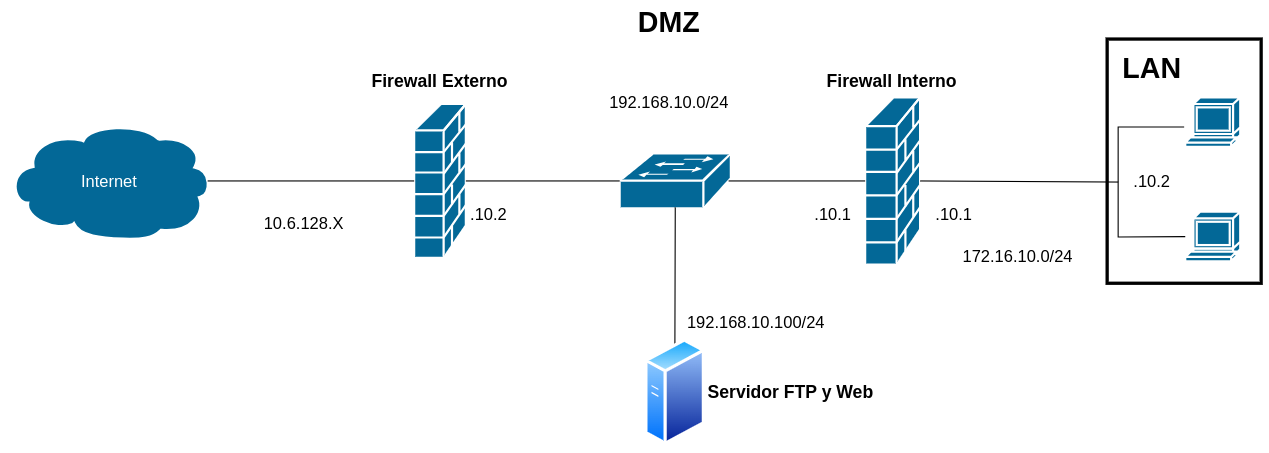
\includegraphics[scale=0.392]{img/esquema_red.png}
  \caption{Diseño de red con dos firewalls y tres zonas}
  \label{fig:Diseno de red con dos firewalls y tres zonas}
\end{figure}

Esta red tendrá tres zonas: \emph{priv} para la red interna, \emph{fw} para el firewall
y \emph{dmz} para la DMZ, con el siguiente direccionamiento:
\begin{itemize}
  \item \textbf{Internet:} la red especificada por el servidor DHCP externo.
  \item \textbf{Red Interna:} Clase C privada como subred de una clase B privada: 172.16.X.0/24.
  \item \textbf{DMZ:} Clase C privada 192.168.X.0/24.
\end{itemize}

% Una vez hecha la configuración de la red, se va a borrar las intefaces externas por defecto
% en el servidor, el cliente y el firewall interno.

\section{Configuración de la red en el firewall externo}
Para la configuración de la red en el firewall externo, se va a configurar la interfaz que
va conectada a la DMZ, para ello se va a configurar el archivo \emph{/etc/network/interfaces}
con la siguiente configuración:
\begin{verbatim}
auto ens4
iface ens4 inet static
        address 192.168.10.2
        netmask 255.255.255.0
\end{verbatim}

Una vez configurada la interfaz, se va reiniciar el servicio de red con el siguiente comando: \\
\begin{BVerbatim}
sudo systemctl restart networking
\end{BVerbatim}

% Nueva página
\cleardoublepage

\section{Configuración de la red en el firewall interno}
Para la configuración de la red en el firewall interno, se va a configurar dos interfaces, una
que va conectada a la DMZ y otra que va conectada a la red interna. Como esta máquina es un \emph{CentOS},
la configuración de la red lo haremos con \emph{nmtui}. Para la instalación de \emph{nmtui}, se va a utilizar
el siguiente comando:
\begin{BVerbatim}
sudo yum install NetworkManager-tui
\end{BVerbatim}

Una vez instalado \emph{nmtui}, se va a configurar la interfaz que va conectada a la DMZ, queda de la siguiente
manera:
\begin{figure}[H]
  \centering
  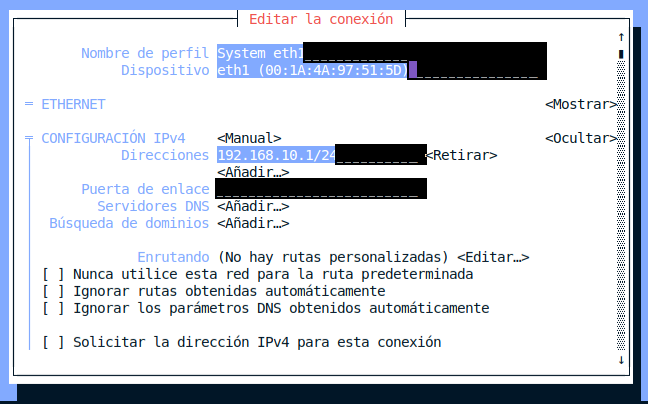
\includegraphics[scale=0.5]{img/fw-interno_to_DMZ.png}
  \caption{Configuración de la interfaz que va conectada a la DMZ}
  \label{fig:Configuracion de la interfaz que va conectada a la DMZ}
\end{figure}

Luego, se va a configurar la interfaz que va conectada a la red interna, queda de la siguiente manera:
\begin{figure}[H]
  \centering
  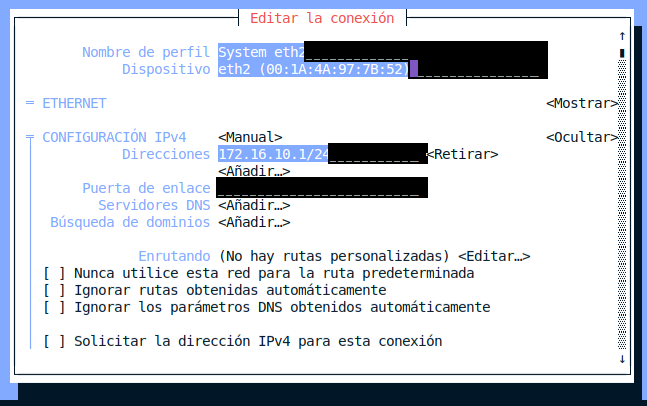
\includegraphics[scale=0.5]{img/fw-interno_to_LAN.png}
  \caption{Configuración de la interfaz que va conectada a la red interna}
  \label{fig:Configuracion de la interfaz que va conectada a la red interna}
\end{figure}

% Nueva página
\cleardoublepage

% Capitulo 2
\chapter{Habilitar \emph{NAT} utilizando la configuración de \emph{Shorewall}}
Para habilitar \emph{NAT} utilizando la configuración de \emph{Shorewall}, se va a 
configurar el archivo \emph{snat} en el directorio \emph{/etc/shorewall/} con la
siguiente configuración:
\begin{figure}[H]
  \centering
  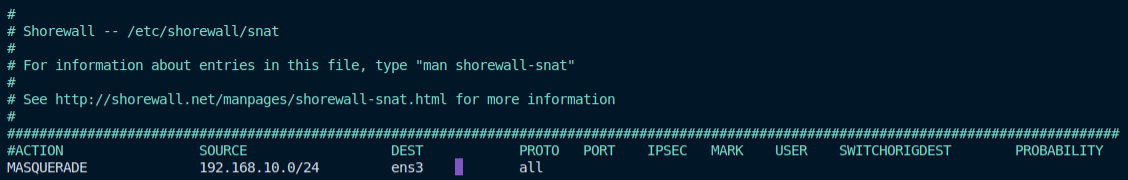
\includegraphics[scale=0.392]{img/snat_config.png}
  \caption{Configuración de \emph{snat}}
  \label{fig:Configuracion de snat}
\end{figure}

% Capitulo 3
\chapter{Configurar el cliente en la red interna y servidor en la DMZ}
\section{Configuración del cliente en la red interna}
Para configurar el cliente en la red interna, se va a configurar el archivo

\section{Configuración del servidor en la DMZ}
Para configurar el servidor en la DMZ, primero se va a instalar el servicio Web
\emph{nginx} con el siguiente comando:
\begin{BVerbatim}
sudo apt install nginx
\end{BVerbatim}

Luego, se va a configurar el archivo \emph{/etc/nginx/sites-available/default} y añadimos
el siguiente contenido:
\begin{verbatim}
server {
  listen 192.168.10.100:80;
  server_name 10.6.128.84;
}
\end{verbatim}

Una vez configurado el archivo, se va a reiniciar el servicio \emph{nginx} con el siguiente comando: \\
\begin{BVerbatim}
sudo systemctl restart nginx
\end{BVerbatim}

Ya con el servicio \emph{nginx} configurado, se va a instalar el servicio \emph{proftpd} para tener un servidor FTP. Para su instalación
se va a utilizar el siguiente comando:
\begin{BVerbatim}
sudo apt install proftpd
\end{BVerbatim}

Con el servicio \emph{proftpd} instalado, se va a iniciar el servicio:
\begin{BVerbatim}
systemctl start proftpd
\end{BVerbatim}
\\ 
\\ 
\\ 
\\
\\
\textbf POR TERMINAR, poner cual es la config de proftpd y pruebas de conexion en ambos servicios

% Nueva página
\cleardoublepage

\chapter{Configurar el firewall con unas políticas por defecto: }



% Nueva página
\cleardoublepage

\chapter{Bibliografía} % En formato APA
\begin{enumerate}
\item Oliveros, D. (2013, 14 de marzo). Configurar Shorewall en Debian. Dayron Oliveros. Recuperado de \url{https://www.youtube.com/watch?v=20E0QxWwAlk}
\item Thomas M. Eastep. (2020). snat — Shorewall SNAT/Masquerade definition file. Shorewall. Recuperado de \url{https://shorewall.org/manpages/shorewall-snat.html}
\item De Luz, S. (2023). Servidor FTP ProFTPd para Linux: Instalación y configuración. Redes Zone. Recuperado de \url{https://www.redeszone.net/tutoriales/servidores/proftpd/}
\end{enumerate}

\end{document}